\documentclass[border=3mm,
               tikz,
               preview,
               qconvert
               ]{standalone}
\usepackage{pgfplots}

\begin{document}

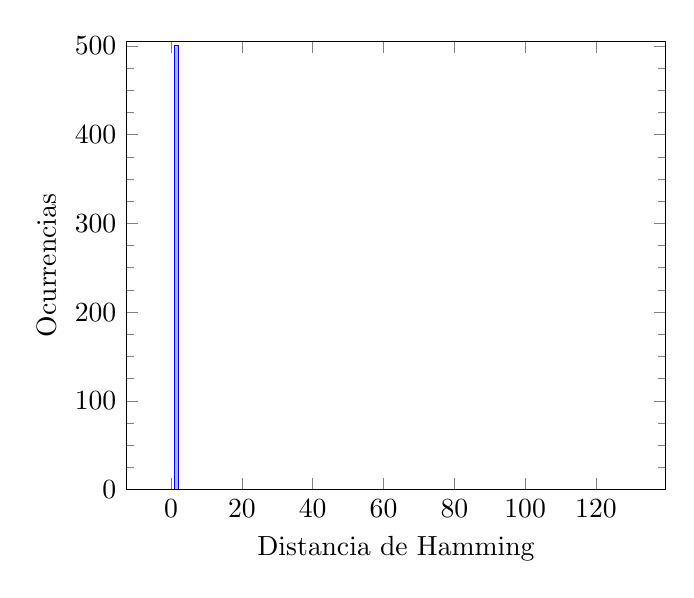
\begin{tikzpicture}
\begin{axis}[
    ymin=0, ymax=505,
    minor y tick num = 3,
    area style,
    ylabel = {Ocurrencias},
    xlabel = {Distancia de Hamming},
    ]
\addplot+[ybar interval,mark=no] plot coordinates { 

(0, 0)
(1, 500)
(2, 0)
(3, 0)
(4, 0)
(5, 0)
(6, 0)
(7, 0)
(8, 0)
(9, 0)
(10, 0)
(11, 0)
(12, 0)
(13, 0)
(14, 0)
(15, 0)
(16, 0)
(17, 0)
(18, 0)
(19, 0)
(20, 0)
(21, 0)
(22, 0)
(23, 0)
(24, 0)
(25, 0)
(26, 0)
(27, 0)
(28, 0)
(29, 0)
(30, 0)
(31, 0)
(32, 0)
(33, 0)
(34, 0)
(35, 0)
(36, 0)
(37, 0)
(38, 0)
(39, 0)
(40, 0)
(41, 0)
(42, 0)
(43, 0)
(44, 0)
(45, 0)
(46, 0)
(47, 0)
(48, 0)
(49, 0)
(50, 0)
(51, 0)
(52, 0)
(53, 0)
(54, 0)
(55, 0)
(56, 0)
(57, 0)
(58, 0)
(59, 0)
(60, 0)
(61, 0)
(62, 0)
(63, 0)
(64, 0)
(65, 0)
(66, 0)
(67, 0)
(68, 0)
(69, 0)
(70, 0)
(71, 0)
(72, 0)
(73, 0)
(74, 0)
(75, 0)
(76, 0)
(77, 0)
(78, 0)
(79, 0)
(80, 0)
(81, 0)
(82, 0)
(83, 0)
(84, 0)
(85, 0)
(86, 0)
(87, 0)
(88, 0)
(89, 0)
(90, 0)
(91, 0)
(92, 0)
(93, 0)
(94, 0)
(95, 0)
(96, 0)
(97, 0)
(98, 0)
(99, 0)
(100, 0)
(101, 0)
(102, 0)
(103, 0)
(104, 0)
(105, 0)
(106, 0)
(107, 0)
(108, 0)
(109, 0)
(110, 0)
(111, 0)
(112, 0)
(113, 0)
(114, 0)
(115, 0)
(116, 0)
(117, 0)
(118, 0)
(119, 0)
(120, 0)
(121, 0)
(122, 0)
(123, 0)
(124, 0)
(125, 0)
(126, 0)
(127, 0)

};
\end{axis}
\end{tikzpicture}
    \end{document}

